\documentclass[a4paper,12pt,UTF8]{article}
\usepackage{ctex}
\usepackage[sort&compress]{gbt7714} 
\usepackage{NUEDCReport}
\usepackage{cite}
\usepackage{enumitem}

\definecolor{c1}{HTML}{2752C9} 
\lstloadlanguages{C}
\lstdefinestyle{Cstyle}{
backgroundcolor=\color{gray!5},
language=C,
frameround=tftt,
frame=shadowbox,
keepspaces=true,
breaklines,
columns=spaceflexible,
escapeinside=``,
basicstyle=\ttfamily\small, % 基本文本设置,字体为teletype,大小为scriptsize
keywordstyle=[1]\color{c1}\bfseries,
keywordstyle=[2]\color{red!70!black},
keywordstyle=[3]\color{teal!70!white},
stringstyle=\color{purple},
showstringspaces=false,
commentstyle=\ttfamily\scriptsize\color{green!40!black},%注释文本设置,字体为sf,大小为smaller
tabsize=2,
morekeywords=[1]{uint8_t,uint16_t,uint32_t},
morekeywords=[2]{fft_proc,adc_data_calc_input, arm_cfft_f32, arm_cmplx_mag_f32,
                find_max_index, find_max, curr_thd_calc, arm_rms_f32, power_calc},
morekeywords=[3]{RESULT_SIZE, VOLT_COEF, COIL_N},
numbers=left, % 代码行数
numberstyle=\it\tiny\color{gray}, % 代码行数的数字字体设置
stepnumber=1,
rulesepcolor=\color{gray!30!white}
}


% 标题格式设置
\titleformat{\section}{\Large\bfseries}{\thesection}{1em}{}
\titleformat{\subsection}{\large\bfseries}{\thesubsection}{1em}{}
\titleformat{\subsubsection}{\normalsize\bfseries}{\thesubsubsection}{1em}{}

\titlespacing*{\section}{0pt}{0.025\baselineskip}{0.05\baselineskip}
\titlespacing*{\subsection}{0pt}{0.025\baselineskip}{0.05\baselineskip}
\titlespacing*{\subsubsection}{0pt}{0.025\baselineskip}{0.05\baselineskip}

% 目录格式设置
\dottedcontents{section}[0em]{\vspace{0.5em}}{1.5em}{0.5pc}
\dottedcontents{subsection}[2em]{}{2.3em}{0.5pc}
\dottedcontents{subsubsection}[4.4em]{}{3.2em}{0.5pc}


% 摘要格式设置
\renewcommand{\abstractnamefont}{\large\bfseries} % 摘要标题字体
\renewcommand{\abstracttextfont}{\normalsize} % 摘要正文字体
\setlength{\absleftindent}{0pt} % 摘要左缩进
\setlength{\absrightindent}{0pt} % 摘要右缩进

% 正文行距设置
\linespread{1.44}

% 开始文档
\begin{document}
\captionsetup{font={small}} % 图表标题字体
\cover
\thispagestyle{empty}
\pagestyle{empty}
% 生成标题页


\newpage
% 生成摘要页
\begin{abstract}
本设计基于 LP-MSPM0G3507 设计了单相功率分析仪。
该系统通过电流互感器和电压互感器实现对用电插座上负载的电流和电压的测量,
系统利用 MSPM0 内部的程控放大器对信号进行放大, 
ADC 进行采集, DMA 传输数据,计算实际的电压、电流。
通过内置比较器检测信号的过零点,并通过一个周期的积分计算平均值
以得出有功功率。同时,系统通过计算电压和电流的均方根值获得视在功率,
并进一步计算功率因数。设计使用 FFT,用于计算电流谐波系数以及 2 至 10 次谐波的有效值。
设计与 PA 测量相对误差绝对值低。此外,系统设计注重低功耗,
充分考虑了电气安全规范。本设计各个模块布局合理,
系统稳定性好,制作成本低。


\noindent \textbf{关键词:} 
MSPM0、程控放大器、比较器、FFT、电流谐波系数
\end{abstract}

% 新起一页
\newpage

% 生成目录页
\tableofcontents

% 新起一页
\newpage
\pagestyle{fancy}
\setcounter{page}{1}
% 开始正文
\section{设计任务与要求}
基于 TI 公司的微控制器(MCU)芯片,设计并制作一个单相功率分析仪。
该系统需测量用电插座上的负载的电流、电压、有功功率、功率因数、电流
总谐波失真(THD)及 2$\sim$10 次谐波分量的有效值。要求测量精度高,
相对误差绝对值:电流、电压及有功功率$\leqslant 1\%$,电流总谐波失真
$\leqslant 2\%$。系统需低功耗,工作功耗$\leqslant 50\mathrm{mW}$,
且采用隔离的电流、电压传感测量方案,确保安全。系统由电池供电。

\section{系统方案设计}
\subsection{设计方案的比较与选择}

\subsubsection{电压互感器方案选型}
方案一:电压输出型电压互感器。电压输出型电压互感器采用电力变压器的原理,
在二次侧输出与一次电压成比例的电压信号,用于高阻抗的输入测量设备。
不能够输出大的电流,通常要使用运放提高输出阻抗后采样。

方案二:电流输出型电压互感器。电流输出型电压互感器通常为 1:1 的电流比例,通过在输入端串联匹配电阻,
输出端并联匹配电阻(实际中通常用运放来把电流信号转化为电压信号)
来实现电压的比例的调整,输出阻抗小,而且为电流信号,不容易受到导线长度的影响。

综合以上两种方案,电流输出型电压互感器输出阻抗小,且能够通过更改匹配电阻方便的修改电压变比,我们选择方案 2。

\subsubsection{电流测量增益控制方案选型}
方案一:使用模拟开关切换比例放大器反馈电阻。使用比例放大电路来放大电流互感器模块的信号,
通过 CD4051 模拟开关来改变比例放大电路的反馈电阻,实现增益控制。反馈电阻可以根据应用自行设定。

方案二:使用 MSPM0 片内程控功放。把电流互感器模块输出的电压信号接入到 MSPM0,通过 MSPM0 的外设 OPA 来调整增益,
同向放大时增益可以设为 2、4、8、16、32。   

由于要使用更大范围变化的增益,综合以上两种方案,我们选择方案 1。


\subsubsection{主控板卡的选择}
方案一: LP-MSPM0G3507。LP-MSPM0G3507 开发套件是基于 MSPM0G3507 的易用型评估模块,
包含在 MSPM0G3507 M0+ MCU 平台上开始开发所需要的全部资源,包括用于编程、调试和功率测量的板载调试探针。

方案二:MSPM0L1306 最小系统板。MSPM0L1306 最小系统板体积小,预留调试器接口,
以及一个用户自定义按键,可用于 DIY 设计开发。

方案三:MSP-EXP432E401Y。MSP-EXP432E401Y 开发套件通过集成以太网和一系列有线通信接口。
MSP432E4 MCU 采用了 120MHz Arm Cortex-M4F CPU、1MB 闪存、256kB SRAM 和
先进的加密加速器,为开发人员提供大量的处理资源,从而实现有线和无线连接栈及处理算法,
开发稳健的以太网解决方案。

由于需要使用功耗更低的 MCU,并能够进行功耗分析,综合以上两种方案,我们选择方案 1。

\subsection{系统整体设计方案}
如\autoref{sys} 所示。系统包含两个互感器,信号调理电路,LP-MSPM0G3507 开发板,电源管理模块及电池组成。
电压和电流互感器采样到的信号经过信号调理电路进行放大,滤波之后进入到 MSPM0 内部 ADC 进行采样,
同时 MSPM0 可以通过控制增益控制电路实现自动增益控制。电源管理模块为 MCU 及运放等芯片提供不同的工作电压,
同时优化功耗。
\begin{figure}[htbp]
    \centering
    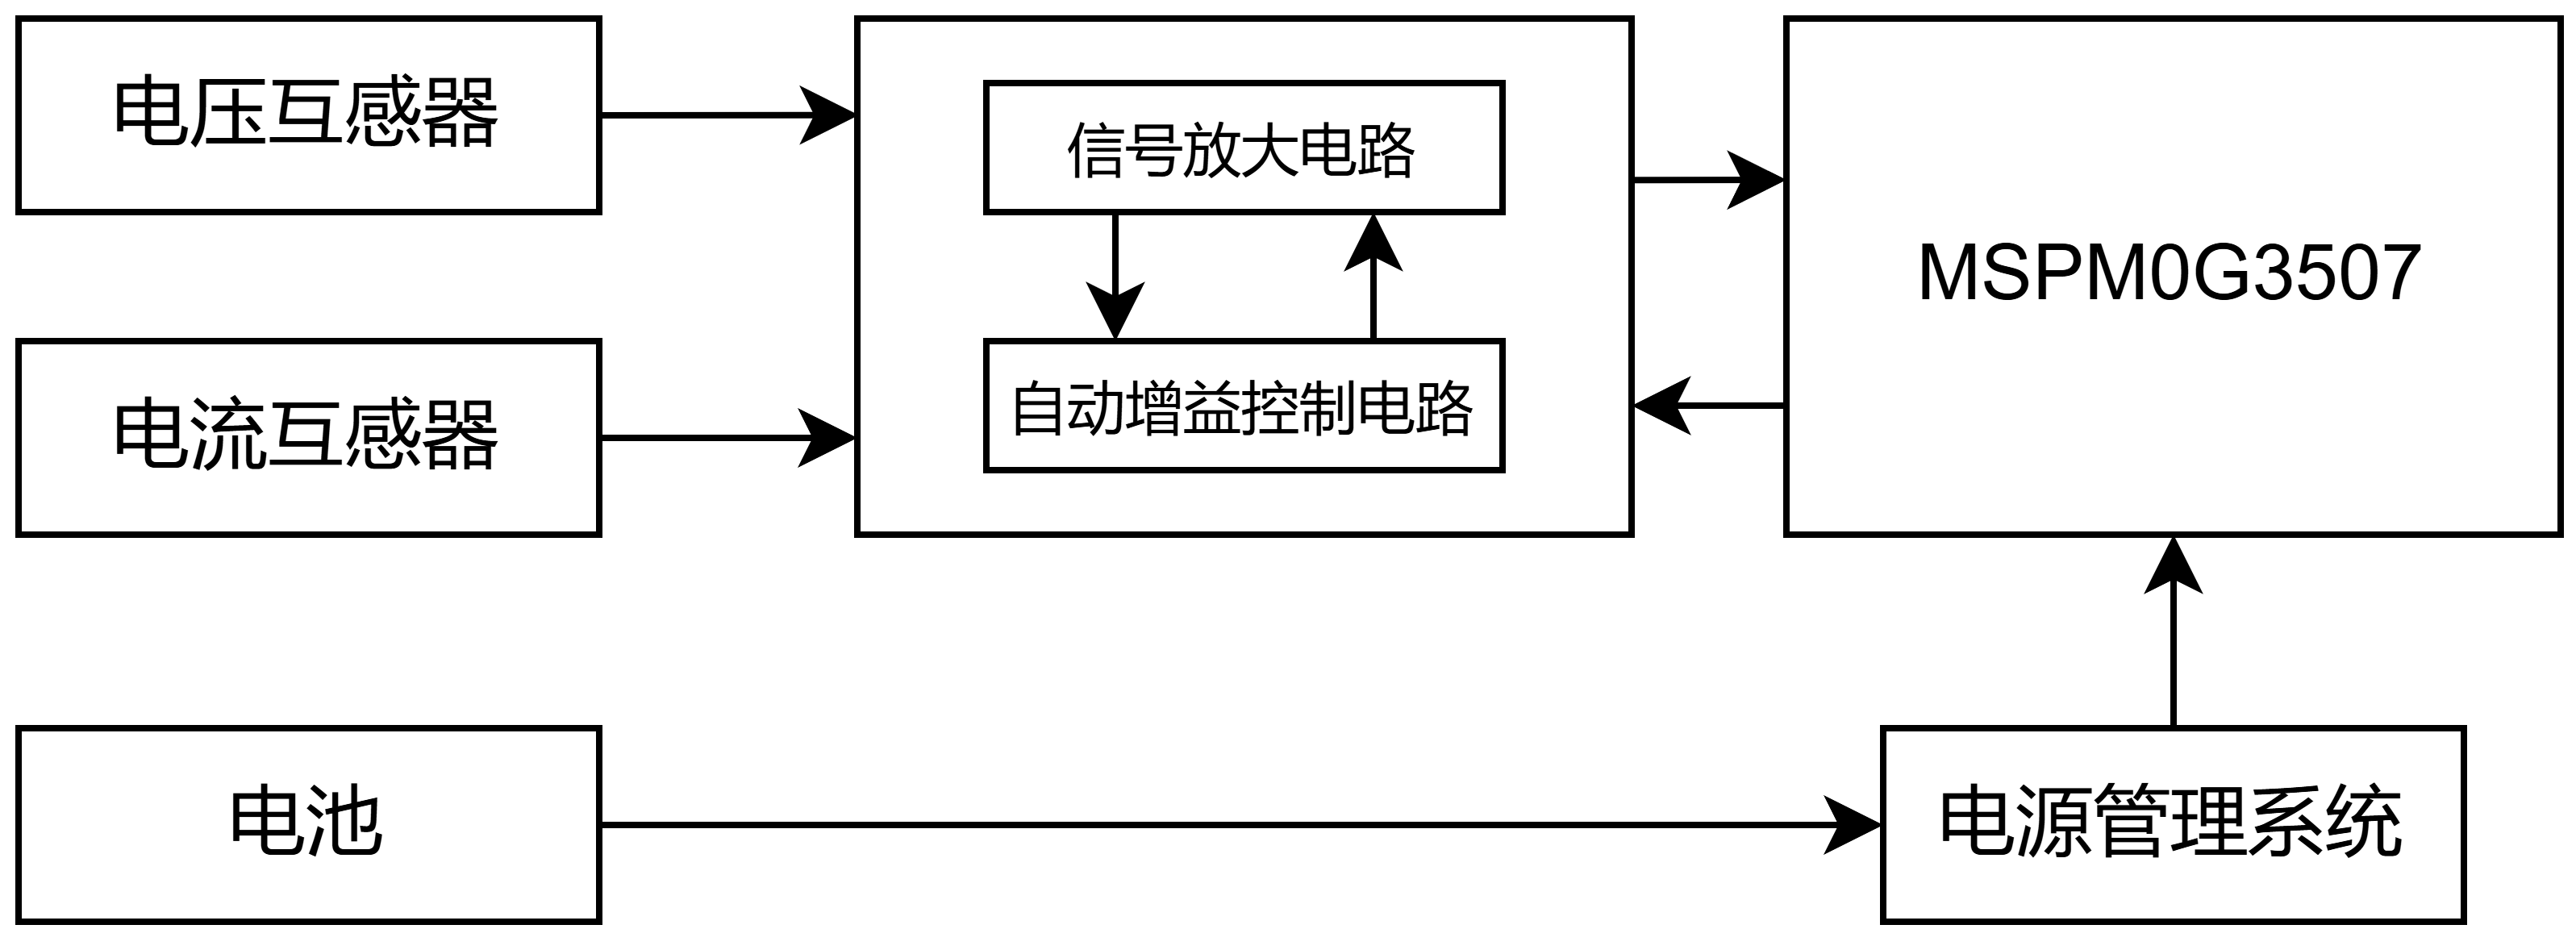
\includegraphics[width=0.6\textwidth]{figures/sys_flowchart.png}
    \caption{系统结构框图}
    \label{sys}
\end{figure}


\section{系统理论分析与计算}
\subsection{交流电参数的计算方法}
电压和电流的采集与转换通过 MSPM0 内部的程控放大器对来自
电压互感器和电流互感器的信号进行放大,确保信号在 ADC 采样范围内。
经过放大的电压和电流信号由 ADC 进行采集。采样频率应合适,
以准确捕捉交流信号的波形。然后利用 MSPM0 内部比较器检测电压
和电流信号的过零点,以确定信号的周期。这对于后续的功率计算和 FFT 分析至关重要。
\subsubsection{有效值计算}
对一个完整周期内采集到的电压或电流数据进行平方、求平均值,然后开平方,如\autoref{eq1} 
和\autoref{eq2} 所示,即可得到电压和电流的均方根值(RMS)。
\begin{equation}
    U_{RMS} = \sqrt{\frac{1}{N}\sum_{i=1}^{N} U_i^2}
    \label{eq1}
\end{equation}
\begin{equation}
    I_{RMS} = \sqrt{\frac{1}{N}\sum_{i=1}^{N} I_i^2}
    \label{eq2}
\end{equation}
其中,$U_i$ 和 $I_i$ 分别为采样点的电压和电流值,$N$ 为一个周期内的采样点数。

\subsubsection{有功功率计算}
通过电压和电流的乘积积分计算有功功率。对于一个周期内的功率,积分结果除以周期得到平均有功功率
如\autoref{eq3} 所示。
\begin{equation}
    P = \frac{1}{N} \sum_{i=1}^{N} U_i \cdot I_i
    \label{eq3}
\end{equation}

\subsubsection{功率因数计算}
功率因数是有功功率与视在功率的比值,如\autoref{eq4} 所示。
\begin{equation}
    PF = \frac{P}{S}
    \label{eq4}
\end{equation}

视在功率利用电压和电流的RMS值计算,如\autoref{eq5} 所示。
\begin{equation}
    S = U_{RMS} \cdot I_{RMS}
    \label{eq5}
\end{equation}

\subsubsection{谐波分析}
对采集的电流信号进行快速傅里叶变换(FFT),提取基波及 2$\sim$10 次谐波的幅值。
通过谐波成分计算电流总谐波失真(THD),如\autoref{eq6} 所示。
\begin{equation}
    THD = \frac{\sqrt{I_2^2 + I_3^2 + \cdots + I_{10}^2}}{I_1}
    \label{eq6}
\end{equation}
其中,$I_1$ 为基波电流,$I_2, I_3, \cdots, I_{10}$ 为各次谐波电流。

\subsection{电流互感器工作原理}
电流互感器是一种用于测量电流的设备。它通过电磁感应原理将高电流转换为低电流,以便安全地测量和监控。
电流互感器有一次绕组和二次绕组。一次绕组通常由被测电路的导线直接穿过互感器的中心,形成一个或少数几个匝数。
二次绕组则绕在铁芯上的多匝线圈,通常有很多匝数。当一次绕组中流过电流时,产生一个磁场,这个磁场在铁芯中产生
磁通。磁通在二次绕组中感应出电压,根据法拉第电磁感应定律,二次绕组中的电压与磁通的变化率成正比。
电流互感器的设计使得一次绕组电流与二次绕组电流之间存在固定的比例关系,称为互感器变比。二次绕组不应在开路
状态下工作,因为开路会导致高电压,可能对设备和人员造成危险。

\subsection{FFT 原理}
快速傅里叶变换(Fast Fourier Transform, FFT)是一种高效计算离散傅里叶变换(DFT)的方法。
DFT 是将时间域的信号转换为频域信号的数学工具,用于分析信号的频率成分。

计算 FFT 主要有以下几个步骤:

输入信号的离散化。输入信号在时间上是离散的,即由一组有限的采样点组成。

分解策略。FFT 的核心思想是通过分而治之的方法将 DFT 计算中的重复部分去除。
具体来说,FFT 通过递归地将一个大规模的 DFT 分解成多个小规模的 DFT,这种分解通常基于信号点数的因子。

蝶形运算。在 FFT 中,最基本的运算单元是“蝶形结构”。蝶形运算将两个点的运算通过一次加法和一次乘法来完成,极大地减少了计算复杂度。

递归计算。通过不断分解,FFT 将复杂度从原始 DFT 的 $O(N^2)$ 降低到 $O(N \log N)$,其中 $N$ 是输入信号的采样点数。

输出结果。最终输出是信号在不同频率下的复数幅度,这些复数值包含了信号的频谱信息,即每个频率成分的幅值和相位。

\section{电路与程序设计}
\subsection{电路设计}
\subsubsection{电压取样电路}
电压取样电路如\autoref{volt_sample} 所示。该电路主要用于测量交流电压,
通过电压互感器将高压信号降到安全的电平,然后通过一系列的滤波和放大电路,
将信号放大到适合后续处理或测量的电平。运算放大器的使用可以提供所需的增益和信号调理,
以确保输出信号的准确性和稳定性。
\begin{figure}[H]
    \centering
    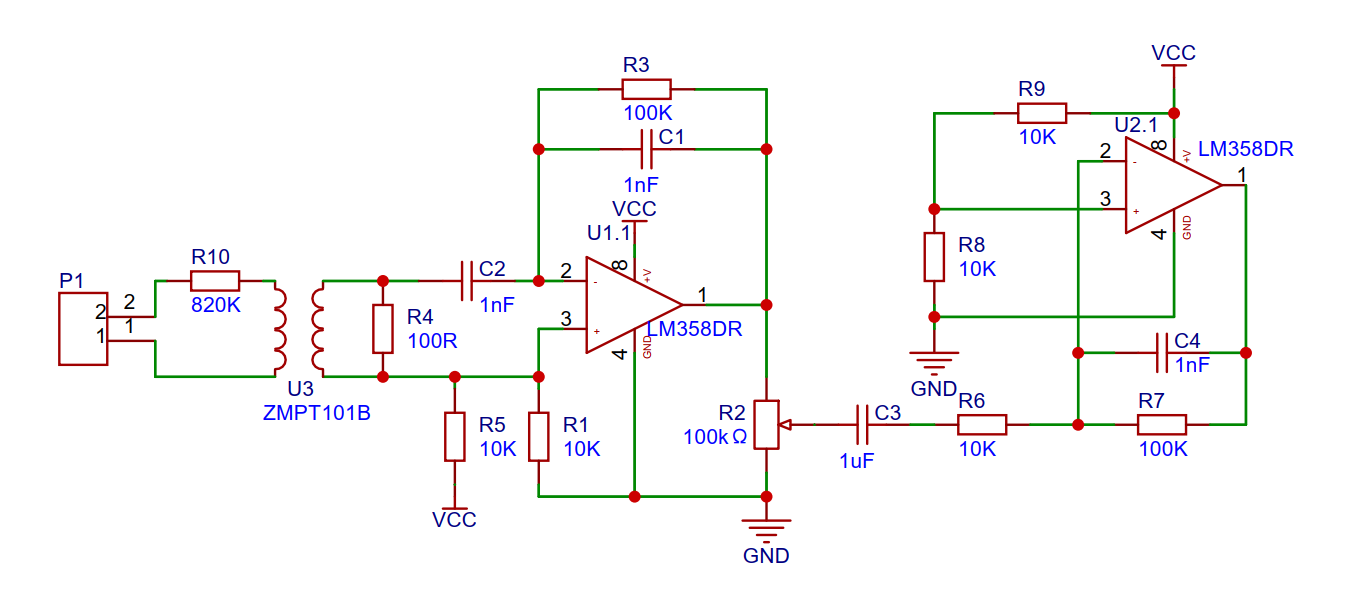
\includegraphics[width=0.8\textwidth]{figures/volt_sample.png}
    \caption{电压取样电路}
    \label{volt_sample}
\end{figure}

\subsubsection{电流取样电路}
电流取样电路如\autoref{curr_sample} 所示。通过电流互感器将高电流信号转换为小电流信号,
再通过电阻将其转换为电压信号。信号经过两级运算放大器的放大和调理,最终输出适合测量或处理的电压信号。
增益控制模块用于动态调整信号的增益,以适应不同的电流测量范围。
\begin{figure}[H]
    \centering
    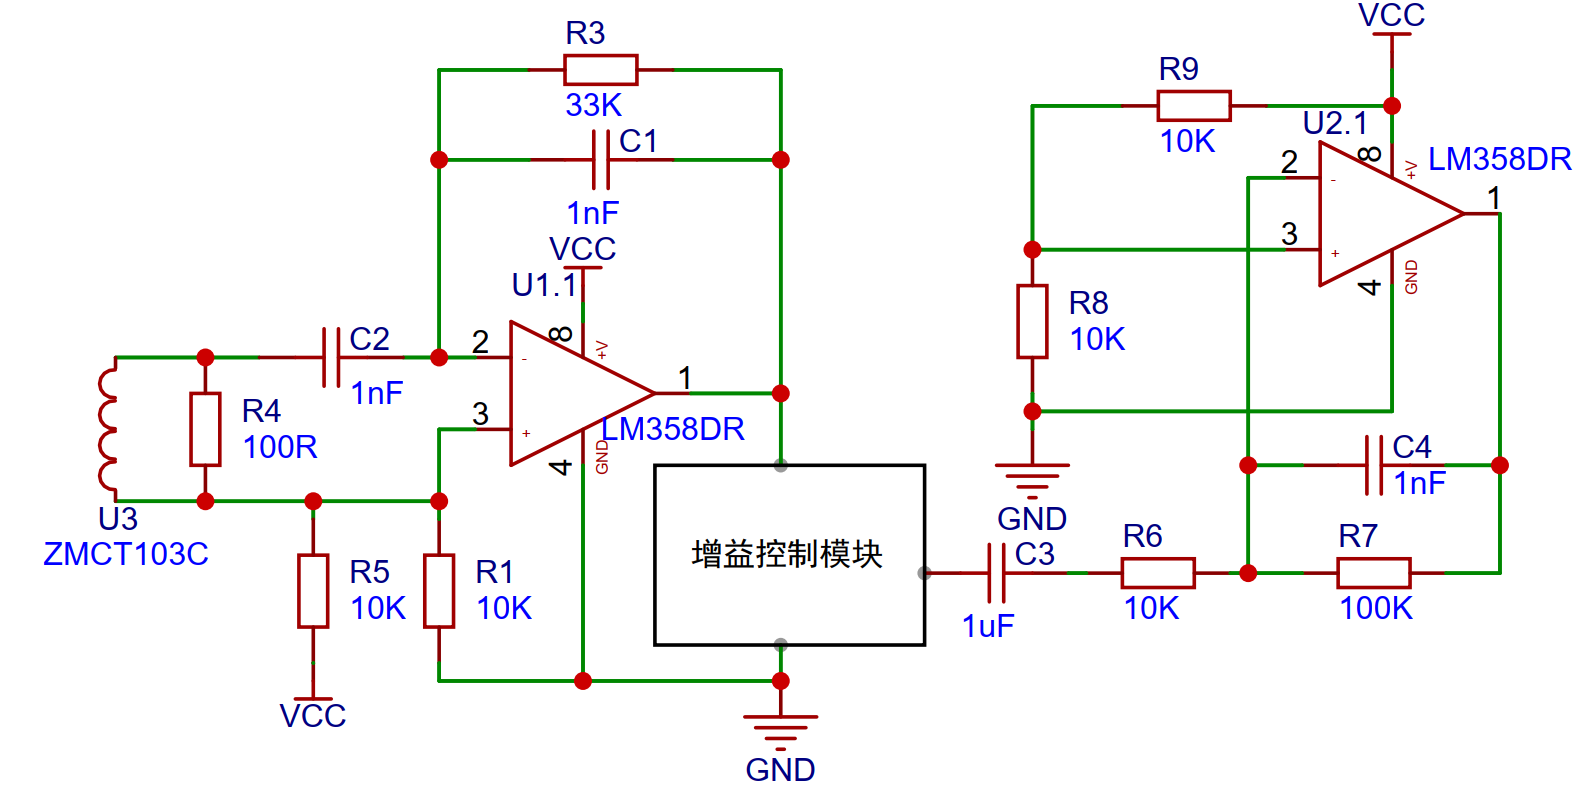
\includegraphics[width=0.6\textwidth]{figures/curr_sample.png}
    \caption{电流取样电路}
    \label{curr_sample}
\end{figure}

\subsubsection{电流增益控制电路}
电流增益控制电路如\autoref{gain_ctrl} 所示。通过使用模拟多路复用器 (CD4051BE) 和一个运算放大器 (LM358DR),
实现了输入信号的可控增益。多路复用器允许选择不同的电阻路径,从而调整输入信号的幅度。
然后,运算放大器根据设定的增益放大信号。通过改变选择信号 (A, B, C),可以动态调整输入信号的增益。
\begin{figure}[H]
    \centering
    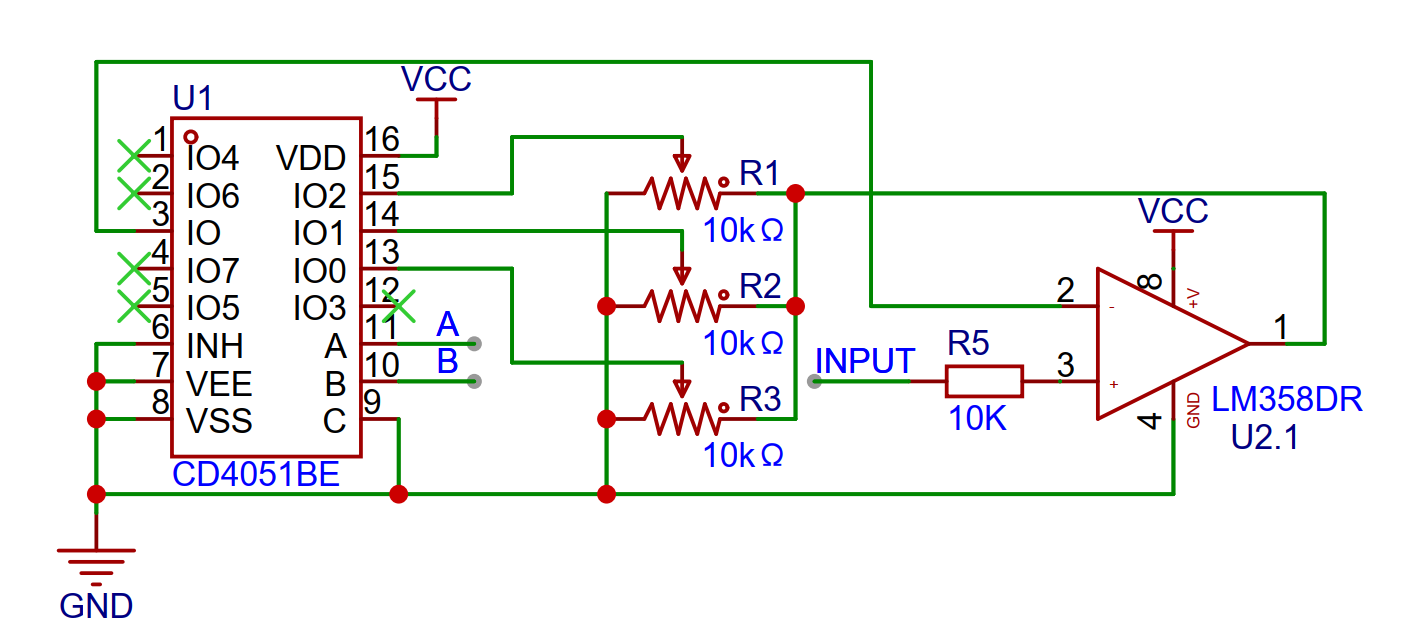
\includegraphics[width=0.6\textwidth]{figures/gain_ctrl.png}
    \caption{电流增益控制电路}
    \label{gain_ctrl}
\end{figure}

\subsection{程序设计}
\subsubsection{整体程序工程流程}
根据题目要求和设计方案,
本文设计了整体程序流程如\autoref{general_flowchart} 所示。
\begin{figure}[H]
    \centering
    \begin{minipage}{0.45\textwidth}
        \centering
        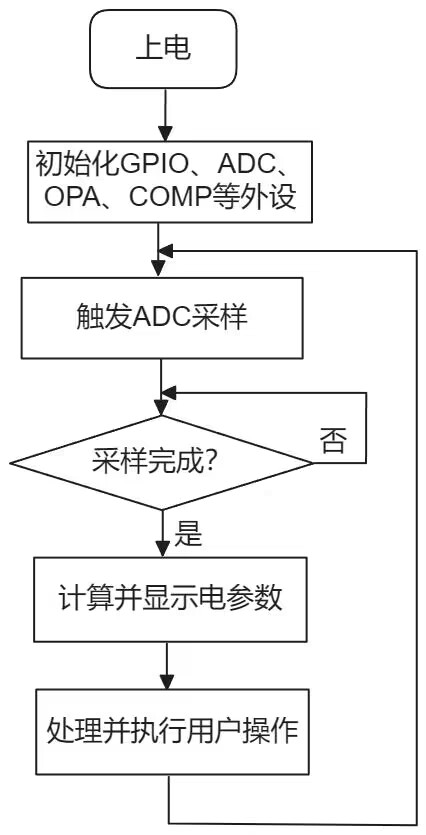
\includegraphics[width=0.45\textwidth]{figures/general_flowchart.jpg}
        \caption{整体程序流程图}
        \label{general_flowchart}
    \end{minipage}
    \quad
    \begin{minipage}{0.45\textwidth}
        \centering
        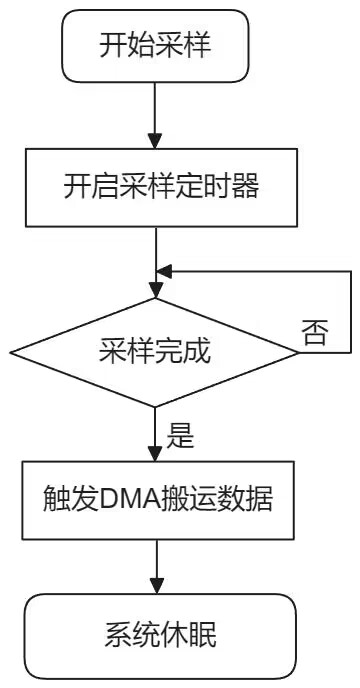
\includegraphics[width=0.45\textwidth]{figures/adc_flowchart.jpg}
        \caption{ADC采样工作流程图}
        \label{adc_flowchart}
    \end{minipage}
\end{figure}

\subsubsection{ADC采样工作流程}
如\autoref{adc_flowchart} 所示,ADC采样工作流程主要包括采样、DMA传输等步骤。
另外为满足低功耗要求,系统在空闲时进入低功耗模式,以降低功耗。


\subsubsection{电流增益自动控制流程}
电流增益设计了三个档位,工作时,先根据ADC采样的数据计算峰峰值,
峰峰值与当前档位的高低阈值行进比较,如果超出当前阈值,就根据超出的方向进行增减档位,
如果没有超出阈值,则保持当前档位增益不变。

\section{系统测试及结果分析}

\subsection{测试方案}
为了验证系统的性能是否满足设计要求,本设计采用了以下测试方案,
使用功率分析仪和设计作品同时对电烙铁、电热锅和 LED 灯管进行分析,计算每测量数据并分析误差。
把电压表和电流表接入到作品的供电电路中,在作品工作的过程中记录电压、电流表的示数,
分析作品功耗。测试仪器见\autoref{tab1}。

\begin{table}[H]
    \centering
    % \begin{minipage}{0.4\textwidth}
    \caption{测试仪器}
    \begin{tabular}{ccc}
        \toprule
        仪器名称 & 型号 & 数量  \\ \midrule
        示波器 & DS2202A & 1\\
        功率分析仪 & TA3331 & 1 \\
        万用表 &  ZT102A & 2
        \\ \bottomrule
        \label{tab1}
    \end{tabular}
\end{table}  
\begin{table}[H]
    \centering
    % \end{minipage}
    % \space
    % \begin{minipage}{0.4\textwidth}
    \caption{测试结果}
    \begin{tabular}{@{}cccccccc}
        \toprule
        测试负载 &   & $U_{RMS}$ & $I_{RMS}$ & $P$ & $PF$ & $THD$ \\ \midrule
        \multirow{3}{*}{电烙铁} &  功率分析仪  & $223.1\mathrm{V}$ & $150\mathrm{mA}$ & $33.35\mathrm{W}$ & $0.997$  & $6.9\%$ \\
         & 设计作品 & $223.2\mathrm{V}$ & $149\mathrm{mA}$ & $33.16\mathrm{W}$ & $0.997$  & $7.0\%$ \\
         & 误差 & $0.04\%$ & $0.6\%$ & $0.5\%$ & $0\%$ & $1.4\%$ \\ \midrule
         \multirow{3}{*}{电热锅} &  功率分析仪  & $222.9\mathrm{V}$ & $2.21\mathrm{A}$ &  $492.11\mathrm{W}$  & $0.999$ &  $1.1\%$ \\
         & 设计作品 & $223.0\mathrm{V}$ & $2.23\mathrm{A}$ & $496.29\mathrm{W}$  & $0.998$  & $1.1\%$ \\
         & 误差 & $0.04\%$ & $0.9\%$ & $0.02\%$  & $0.01\%$  & $0\%$ \\ \midrule
         \multirow{3}{*}{LED 灯管} &  功率分析仪  & $223.6\mathrm{V}$ & $101.33\mathrm{mA}$ &  $18.76\mathrm{W}$  & $0.828$ &  $8.5\%$ \\
         & 设计作品 & $223.4\mathrm{V}$ & $102.01\mathrm{mA}$ & $18.68\mathrm{W}$  & $0.819$  & $8.3\%$ \\
         & 误差 & $0.08\%$ & $0.06\%$ & $0.04\%$  & $1\%$  & $2\%$ \\ \bottomrule
        \end{tabular}
    \label{tab2}
    % \end{minipage}
\end{table}

% \newpage
\subsection{测试结果及分析}
系统的性能经过测试,和成品功率分析仪相比,具有较高的精度;工作状态下的功耗
仅为 $42\mathrm{mW}$,功耗较低,满足题目需求,测试结果见\autoref{tab2} 及附录图 \ref{res}。

\section{结论}
在本次大赛中,我们使用 MSPM0 设计了一个高精度、低功耗的功率分析仪,
能够对交流负载的各种电参数进行分析,满足题目的需求。同时,
我们充分发挥了 MSPM0 MCU 的优势,使用了片内运放、比较器等模拟外设,
简化了外部电路。我们通过降低主频、关闭无用外设、休眠 CPU 等方式,
有效的降低了系统功耗。同时,由于比赛时间紧,任务多,我们的作品还
有很多值得改进的地方,比如用户操作逻辑还可以进一步优化,功耗还能
进一步降低。这些都是值得探索的方向。本次比赛,我们学到了许多知识,
激发了我们对于电子的热爱,将引导我们在这个方向上进一步钻研,
为以后的学习铺下道路。

\phantomsection
\addcontentsline{toc}{section}{参考文献} 
\reference


\newpage

\appendix
\section{附录}
\subsection{部分程序代码}
\subsubsection{FFT 计算}
\begin{lstlisting}[style=Cstyle]
    void fft_proc(float *input_signal)
    {
        float input_cmplx[2048]={0};
        for (uint16_t i = 0; i < 1024; i++){
            input_cmplx[2*i] = input_signal[i]*hamming[i];
        }

        arm_cfft_f32(&arm_cfft_sR_f32_len1024 , input_cmplx , 0 , 1);
        arm_cmplx_mag_f32(input_cmplx,volt,1024);

        uint16_t base_wave_index=find_max_index(volt,3,20);
        harmonic[1]=find_max(volt,3,20)/512;
        for(uint16_t i=2;i<16;i++){
           harmonic[i]= find_max(volt, base_wave_index*i-3, base_wave_index*i+3) / 512;
        }
        curr_thd_calc();
    }
\end{lstlisting}

\subsubsection{交流电参数计算}
\begin{lstlisting}[style=Cstyle, name=calc]
    static void adc_data_calc_input()
    {
        for (uint16_t i = 0; i < RESULT_SIZE ; i++) {
            volt[i] = volt[i]*VOLT_COEF;
            curr[i] = curr[i]*gain_coef[current_range]/COIL_N;
        }

        arm_rms_f32(volt+volt_edge_inx[0], volt_edge_inx[volt_edge_rec-1]-volt_edge_inx[0]+1, &volt_rms);
\end{lstlisting}
\begin{lstlisting}[style=Cstyle, name=calc]
        arm_rms_f32(curr+volt_edge_inx[0], volt_edge_inx[volt_edge_rec-1]-volt_edge_inx[0]+1, &curr_rms);

        AP=power_calc();
        PF= AP/(volt_rms*curr_rms);
    }
\end{lstlisting}

\subsection{测试结果图}\label{res}
\begin{figure}[H]
    \centering
    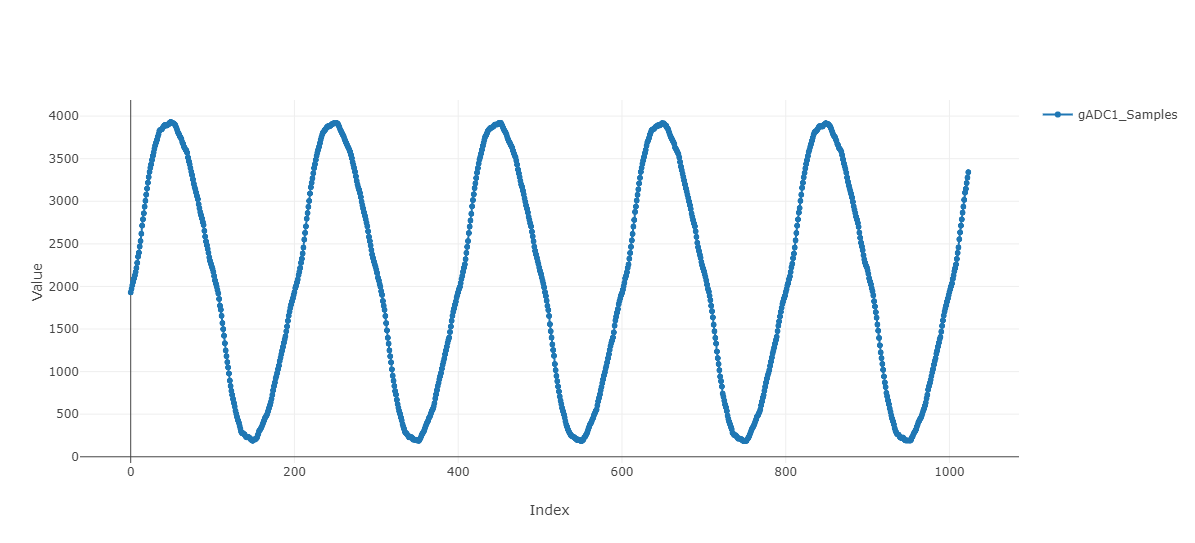
\includegraphics[width=0.7\textwidth]{figures/adc.png}
    \caption{ADC 采样结果}
\end{figure}
\begin{figure}[H]
    \centering
    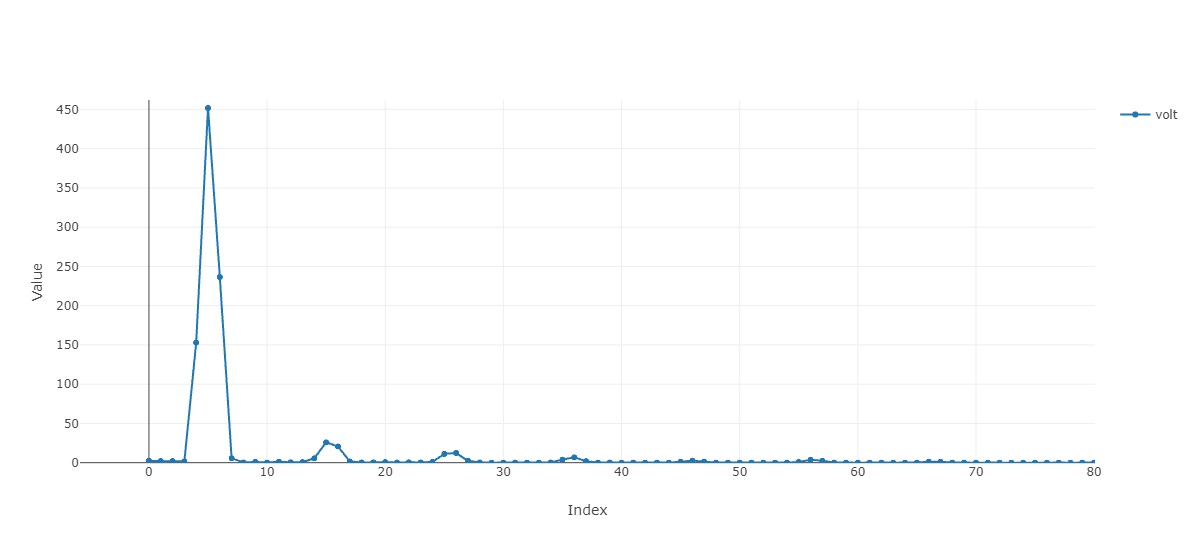
\includegraphics[width=0.7\textwidth]{figures/volt_fft.png}
    \caption{FFT 分析结果}
\end{figure}


% 结束文档
\end{document}
